\documentclass{article}
\usepackage[utf8]{inputenc}
\usepackage[margin=1in]{geometry}
\usepackage{graphicx}
\usepackage{amsmath,amscd}

\begin{document}
\title{Reliable Vertex Connection Methods within One C-Layer}
\maketitle

\begin{enumerate}
\item {\bf Augmented Raster Scan: a reliable method to connect vertices within one layer}\\
\begin{enumerate}
\item Current Implementation\\
In the previous implementations of Raster Scan method, after getting the collision-free line segments, the x-coordinate of two end points $P_L$ and $P_U$, and the middle point $P_M = (P_L + P_U) / 2$ and the corresponding y coordinate are stored in a ``cell'' data structure. The middle points are considered to be ``vertices'' in the roadmap within one layer. To determine if two vertices (i.e. one in $i$th sweep line, and the other in $i+1$th line) can be connected, one must ensure that either one of $P_L$, $P_U$ and $P_M$ in $i$th sweep line is within the range of the collision-free line segment in $i+1$th line, or vice versa. However, the problem occurs when there is an obstacle between the adjacent lines. In this case, the above condition can be satisfied, but since the collision-free area is not convex, sometimes the connecting line would pass through the obstacle between the two sweep lines. We modified this kind of problem as follows.

\begin{figure}
\centering
\label{fig:path_incorrect}
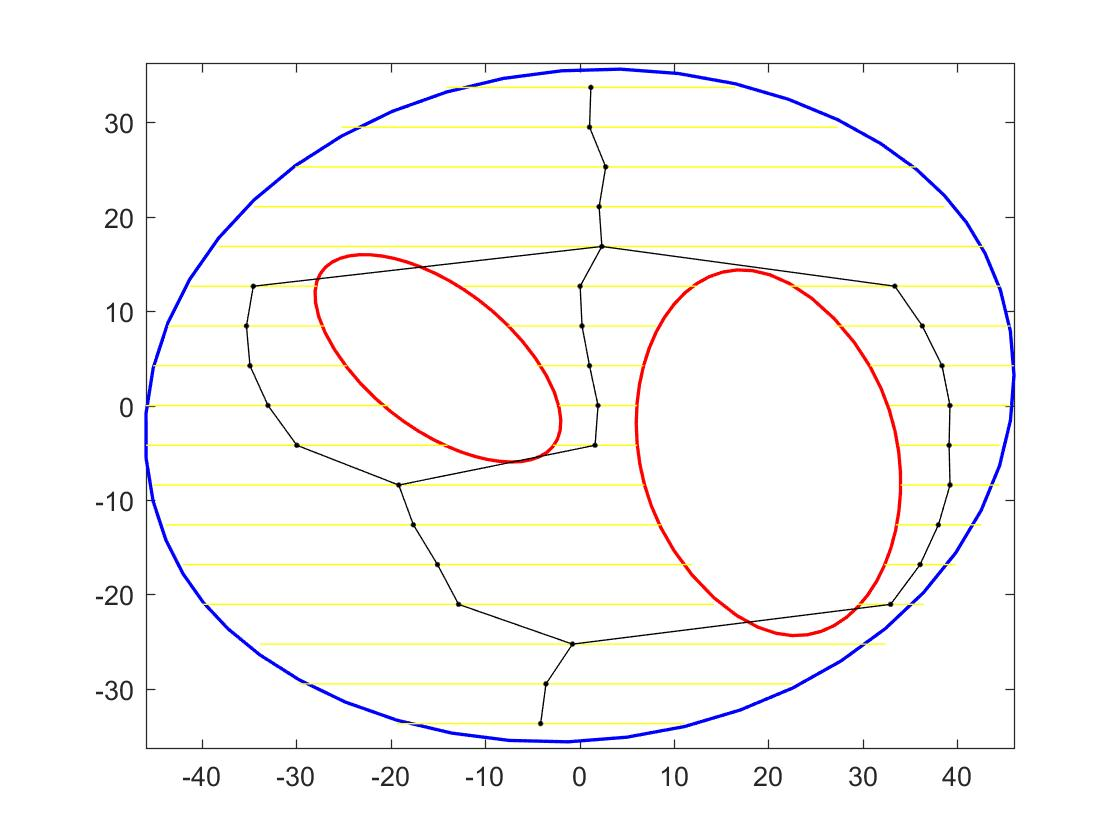
\includegraphics[scale = 0.2]{IncorrectConnection_OneLayer.jpg}
\caption{Incorrect connections.}
\end{figure}

It has been observed that when $P_{Mi}$ (denoting the middle point on the $i$th sweep line) is out of the range of the line segment in the $i+1$th line ($P_{Mi} < P_{Li+1}$ or $P_{Mi} > P_{Ui+1}$), it is dangerous to connect the two vertices ($P_{Mi}$ and $P_{Mi+1}$) with a straight line. So, if this situation occurs, we add another vertex on the $i$th sweep line, whose x-coordinate is equal to $P_{Li+1}$ ($P_{Ui+1}$) if $P_{Mi} < P_{Li+1}$ ($P_{Mi} > P_{Ui+1}$). Note that the previous conditions of determining the connectivities should also be satisfied. As a result, the new augmented method generates a local convex area (a triangle area with the newly generated vertex, the old middle point and one end point in $i+1$th line) within the collision-free area between two sweep lines. And so connecting between the old and new vertices is safe. 

\begin{figure}
\centering
\label{fig:path_oneLayer}
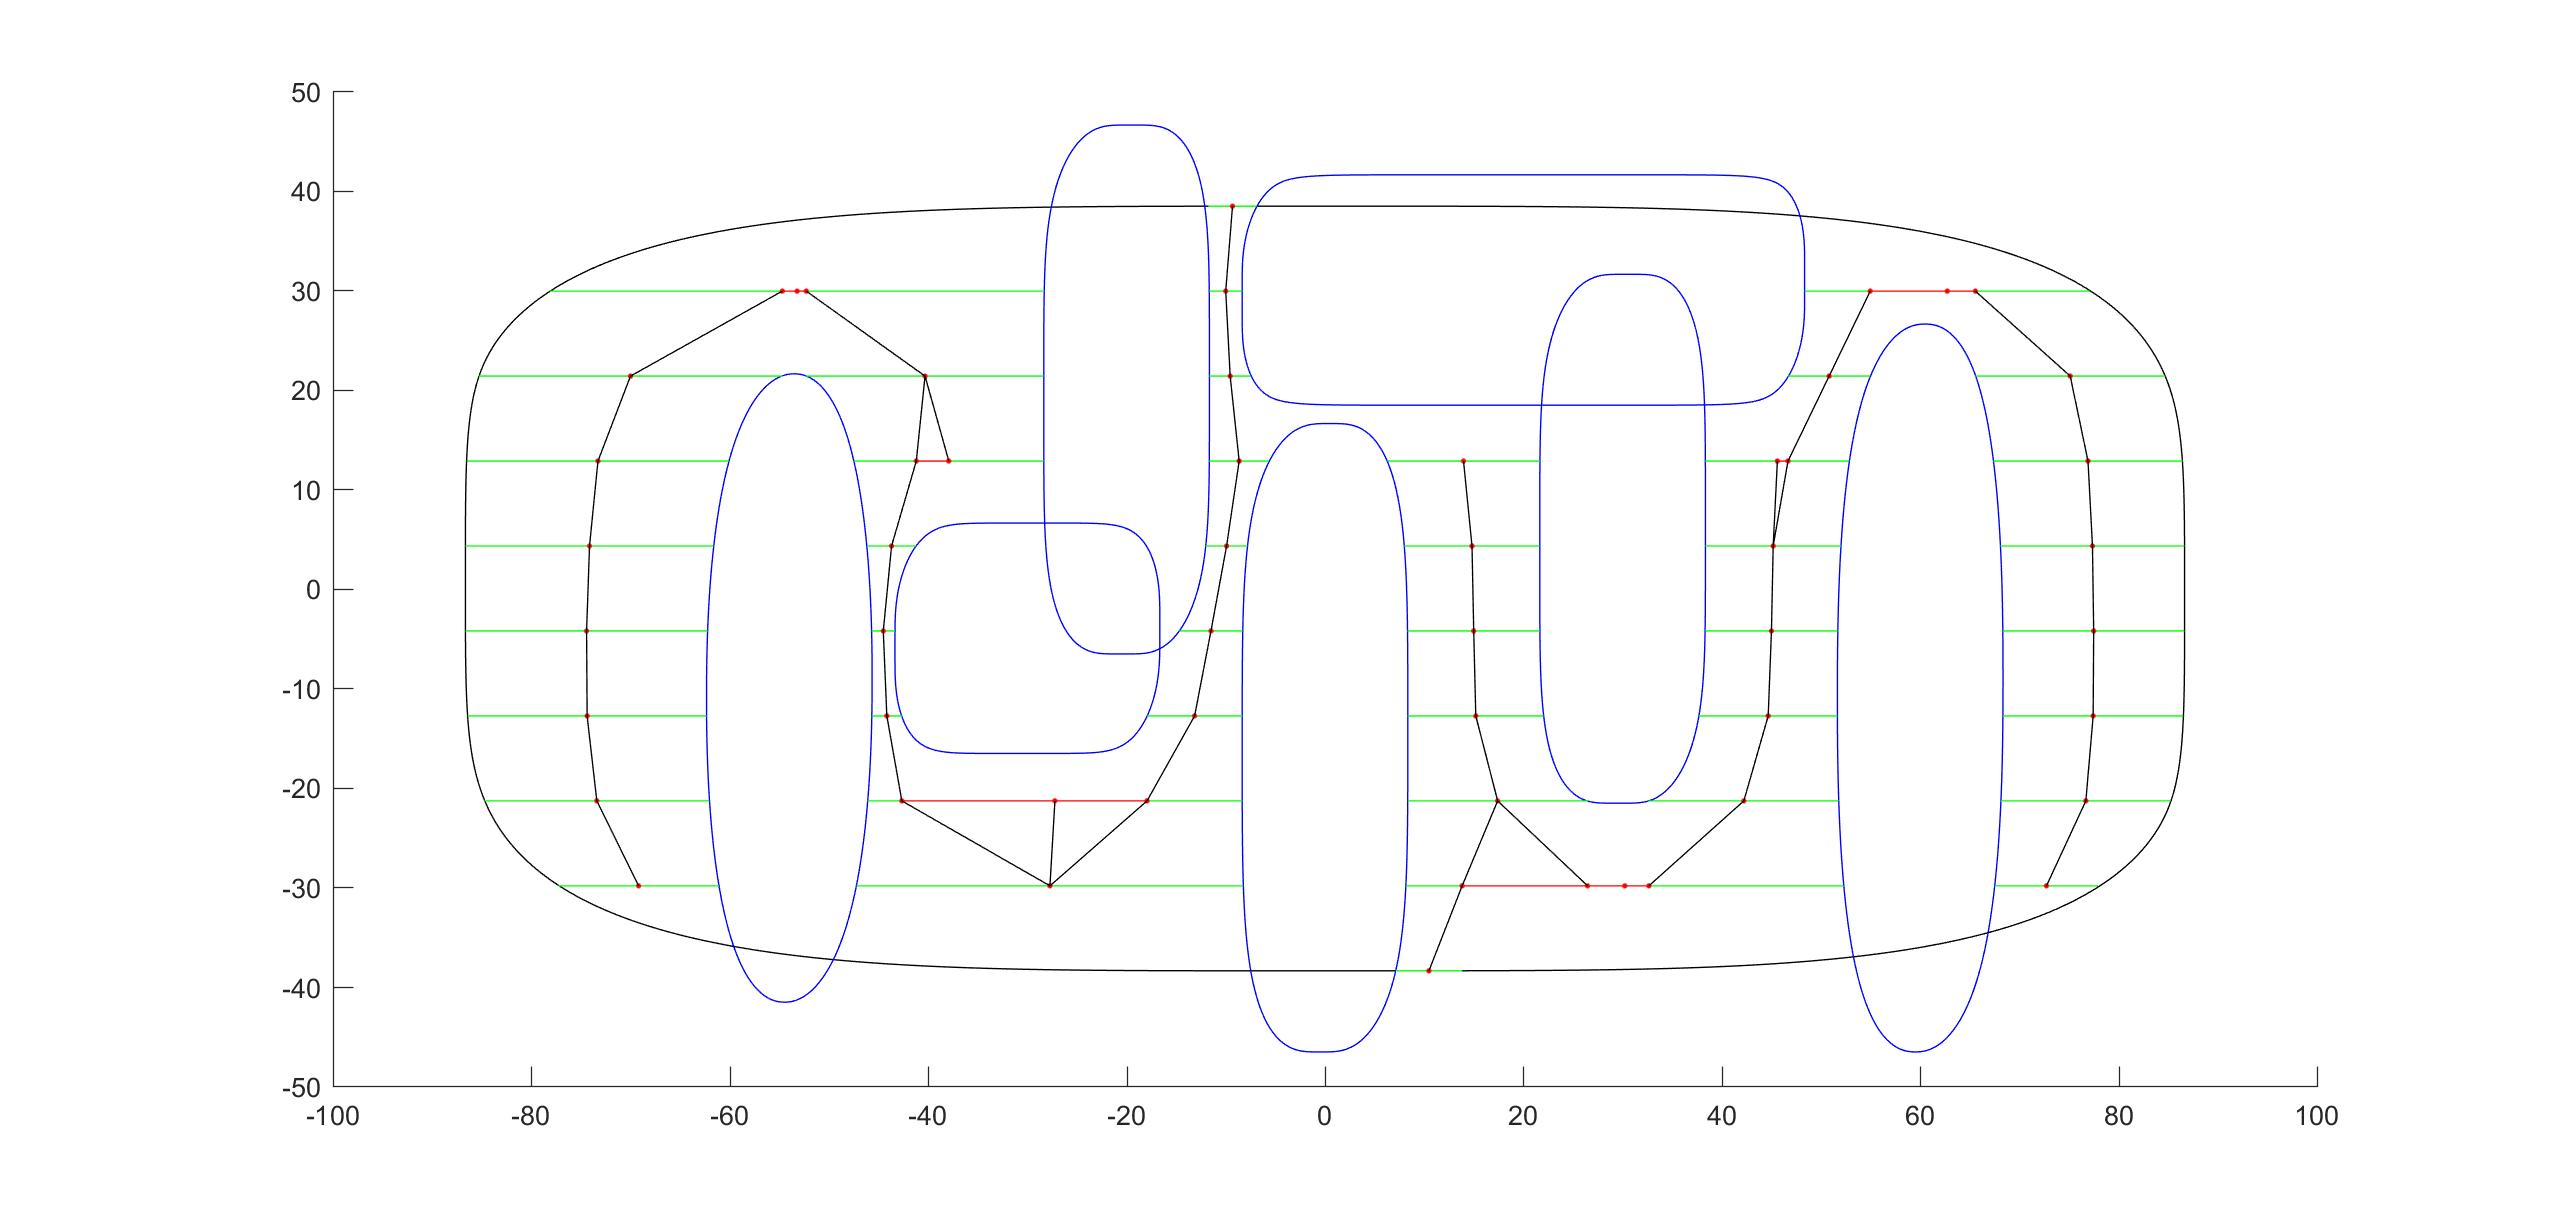
\includegraphics[scale = 0.2]{path_oneLayer.jpg}
\caption{Paths within one layer with augmented raster scan method. Blue: obstacle; Green: sweep lines; Red and Black: safe connections.}
\end{figure}

\item Ideas for further modifications\\
The advantage for the Augmented Raster Scan method is that it decomposes the free space with locally convex cells, providing a reliable vertex connection scheme. With this knowledge, we could further divide the free space with less sweep lines, after which we could further decrease the time for cell decomposition.

The basic idea is to find the left and right most points for each obstacle, and generate the sweep lines using their y-coordinates. To implement this, we just need to find the points with maximum curvature in x direction for each obstacle, and for ellipsoid body, it should return two solutions, which are desired points. This idea can reduce the number of sweep lines (totally $2N$ lines, where $N$ is the number of obstacles), as a result reduce the number of vertices on the roadmap, which in the end reduce the time to construct the roadmap. The drawback is also obvious, one of which is that it throws away a large portion of the free space for the purpose of constructing locally convex cells. 

\end{enumerate}
\newpage

\item{\bf C-Obstacles Boundary Enlargement for generating Convex Collision-Free Cells within one C-Layer}\\
Since the boundaries of C-obstacles generated by Minkowski sums are convex, when using the proposed Raster Scan technique to decompose the C-space, collision-free cells that are between obstacles are concave. Although when the sweep lines are fine enough, curves can be approximated as straight line segments, it is still not safe to connect vertices inside a theoretically concave collision-free cell. To seek for a truly safe cell decomposition, we proposed a procedure to enlarge the C-obstacles to polygons using the intersecting points between the sweep lines and the original C-obstacles as references.

The idea is to find the tangent line of the c-obstacle boundary which is parallel to the line segment determined by two reference points from adjacent sweep lines, and get new points which are intersections between the tangent line and two adjacent sweep lines. We then encapsulate the original c-obstacle with all the newly obtained points to form a polygon, which can be used to further decompose the collision-free c-space.

The new point on each sweep line can be found by adding an offset distance to each reference point, which can be done by first calculating the maximum distance from a point on the boundary to the line segment defined by two reference points, and applying trigonometry to convert into the parameter of the reference point. We first divide the c-obstacle boundary into left and right parts according to the two extreme points that the sweep lines can reach. We then do a search on each part of the divided boundary to find the maximum distance between a point $P = [x, y]^T$ on that part within the range of the reference points $P_1 = [x_1, y_1]^T$ and $P_2 = [x_2, y_2]^T$ (i.e. without loss of generality, assume $y_1 < y_2$, then $y \in (y_1, y_2)$) and the line segment defined by them. The distance from $P$ to the line $l_{P_1P_2}$ defined by $P_1$ and $P_2$ is
\begin{equation}
	d = \frac{\| (y_2-y_1)x - (x_2-x_1)y + x_2y_1 - y_2x_1 \|}{\sqrt{(y_2 - y_1)^2 + (x_2 - x_1)^2}}
\end{equation}

Once the maximum distance is found, we calculate the offset distance as
\begin{equation}
	x_{offset} = \frac{d}{\sin(\theta)}
\end{equation}
where $\theta = atan2 (y_2-y_1, x_2-x_1)$.

At last, we get the new points for each part as follows: for the left part, we subtract the offset distance from the reference point, whereas for the right part, we add such offset distance to make the new point away from the c-obstacle. For each sweep line, i.e. $L_i$ for $i-th$ sweep line, we can get two new points, from $P_{i-1}$ and $P_{i}$, where $P_i$ indicates the reference point on $L_i$, and from $P_i$ and $P_{i+1}$. To eliminate such conflict, we preserve the point that is further from the c-obstacle.

Fig. \ref{BdExplode} shows the result of enlarging the original curved c-obstacle into new polygonal c-obstacle. Fig. \ref{CFArea} shows the convex collision-free c-space in one sample layer.

\begin{figure}
	\centering
	\label{BdExplode}
	\includegraphics[scale = 0.4]{BoundaryExplosion.png}
	\caption{Illustration of enlarging the c-obstacle boundary. Blue curve: actual obstacle boundary; red curve: c-obstacle boundary; black dots: reference points, which are intersections between sweep lines and c-obstacle boundary; red and green dots: new points, which are intersections between the tangent lines and sweep lines; green line segments: enlarged c-obstacle boundary.}
\end{figure}

\begin{figure}
	\centering
	\label{CFArea}
	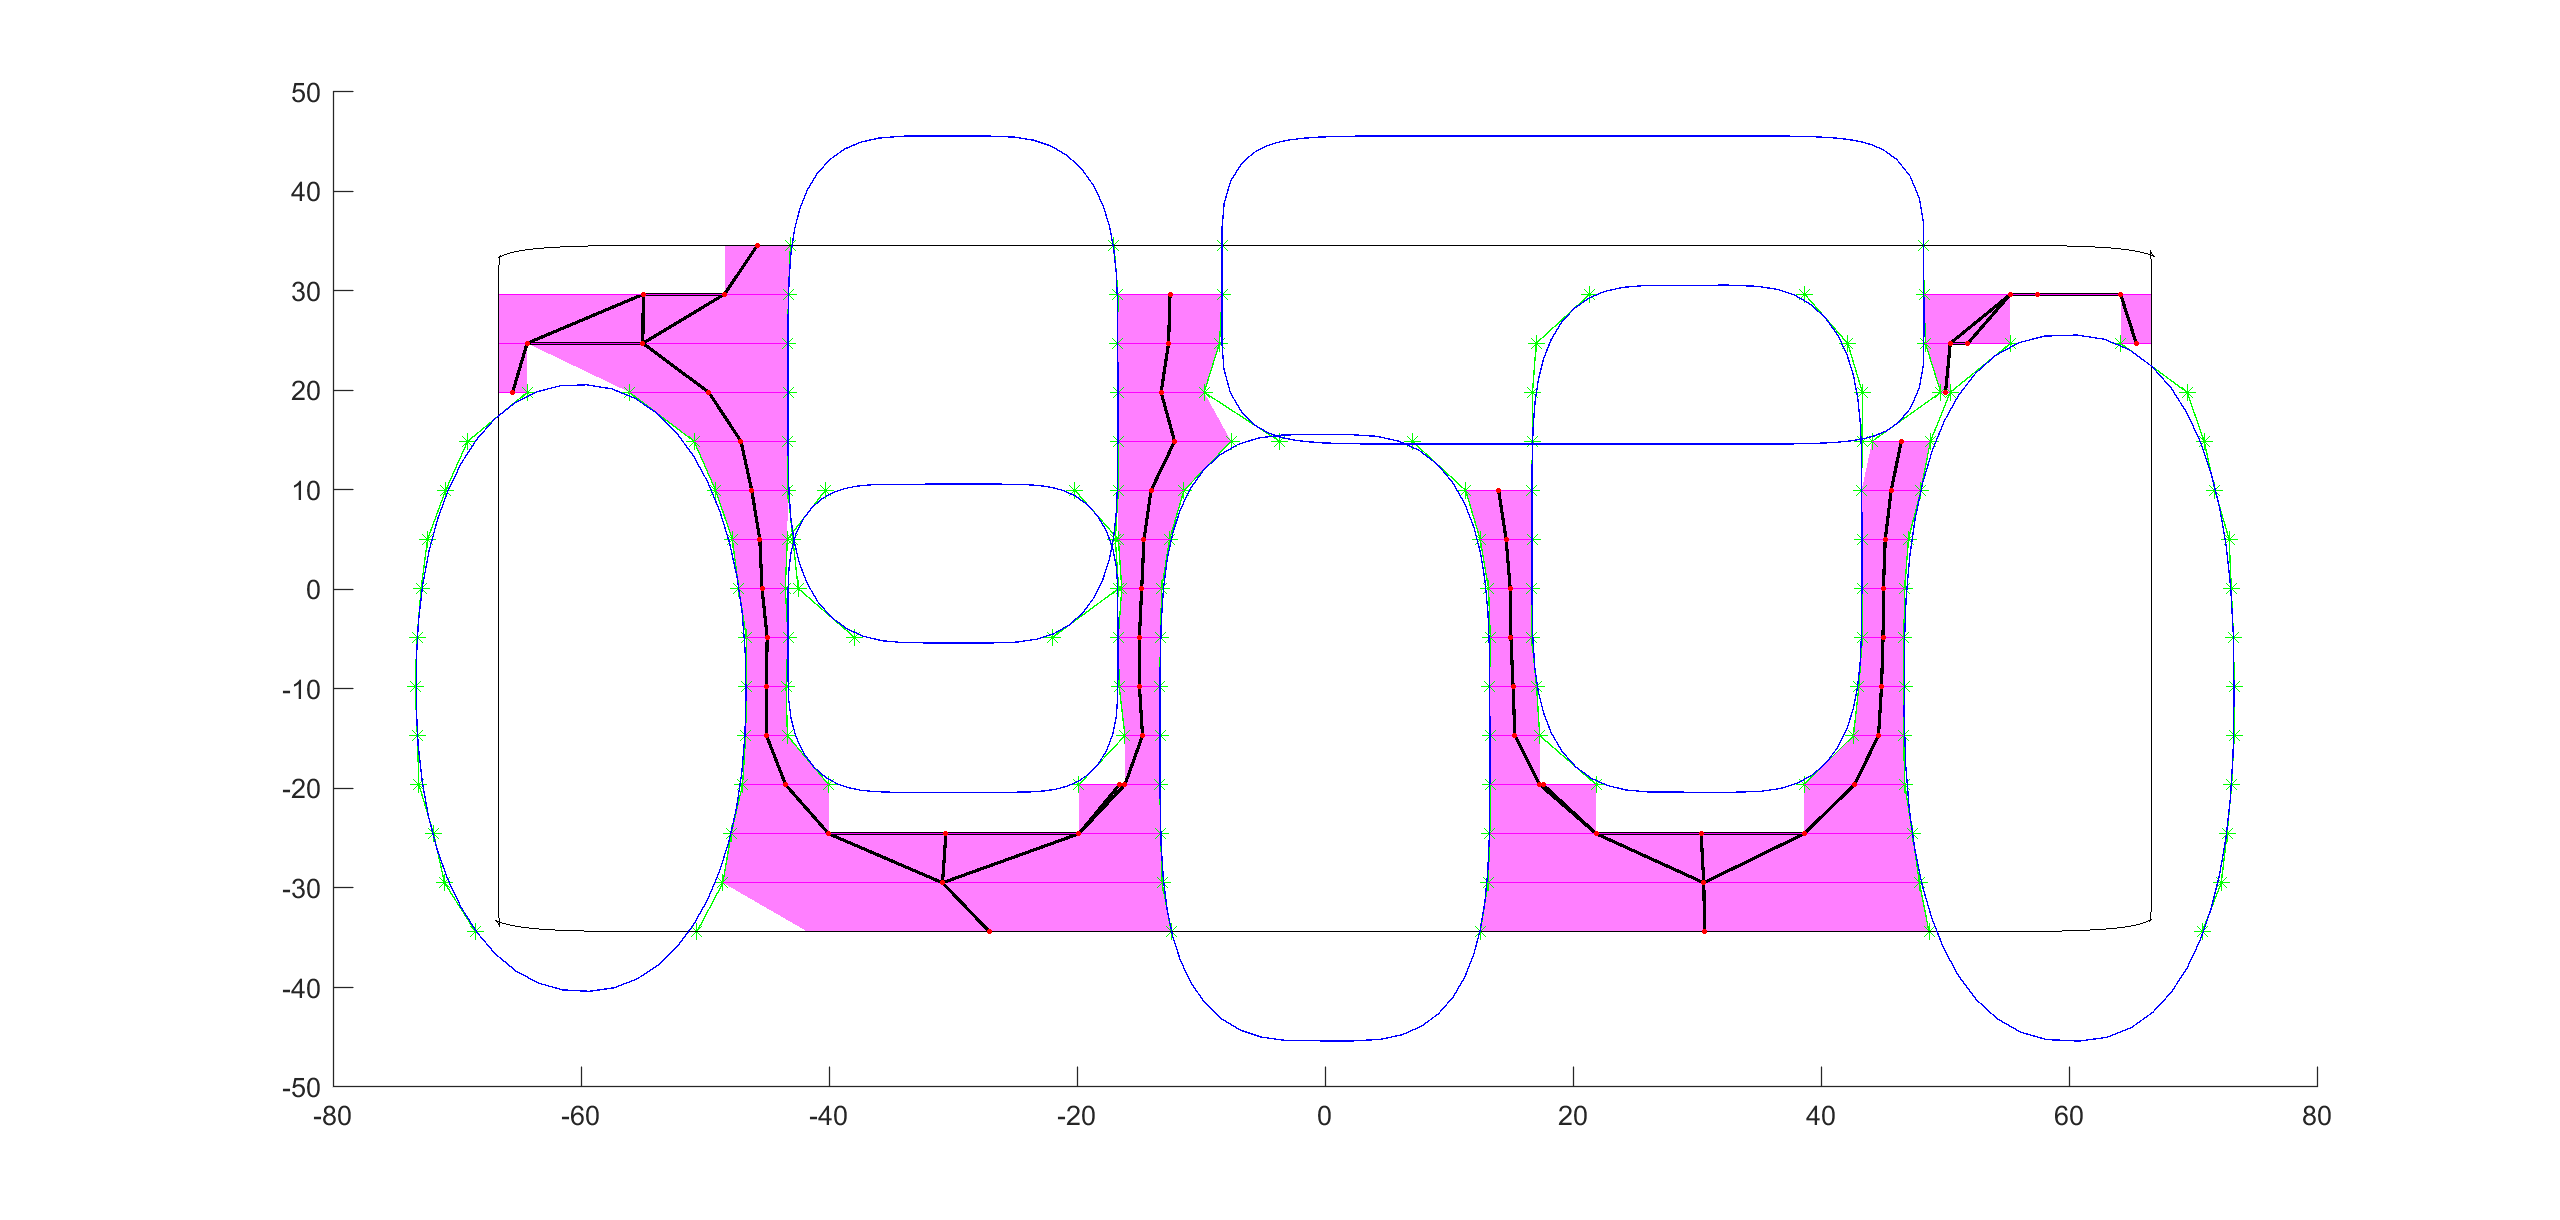
\includegraphics[scale = 0.2]{HighwayWithFreeSpace15.png}
	\caption{Collision-free c-space after enlarging the curved c-obstacles into polygons. Magenta area: convex collision-free c-space.}
\end{figure}

\end{enumerate}
\end{document}
